\chapter{Convolutional neural networks}
As convolutional layers are complex and have many variations for differnet use cases, only concepts and functionaslities that are relevant for this work will be covered. This also menas that 3 dimensional cnns will not be explained, but in generel cnns function the same way whether they have 1, 2 or 3 dimensions. The main differnce lies in how the filter, also known as kernel or festure detector, moves acrross the data. This is later explained in more detail. (\todo{ich glaube input data ist keine regel sondern nur meist so..zum beispiel kann man auch 1d convoltion bei 1d, 2d, oder 3d daten machen}). \\
 First of all the core concepts of cnns will be explained and afterwards the models used in this work will be described.\\

On of the core concepts of convoluntional neural networks are the concolutions. \\




Unituitievly, a 2d cnn must not neccerailty have 2 dimensional data as input.

notes bei models:\\
- stride = wie viele schritte auf einmal, default 1 deshalb vermute ich bei mir 1\\
- maxpooling: pool size = 2*2, und bei keras wird stride dann defauklt auch zu 2*2 (=pool size)\\
- input size = 85*40 glaube ich\\
- filter weights are randomly initialized, so that they dont all initially learn the same feauters. To briefly explain the behaviour of filters a seperation bettween two cases can be made: The first case is that not all features of high quality have been learned yet, high quality meaning that learning them would lower the cost function. In that case it is highly unlikely that each filter would begin to resemble other filters, as that would most certainly result in an increase of the cost function and therefore no gradient descent algorithm would head in that direction. The other case is that all features of high quality have already been leanred by a subset of the avaibable filters. In this case the cost function would not be increased if the remaining filters learn similar features than the other filters. \\
- in einem der schritte wird eine zeile usgelassen, aber ich trainiere nicht nochmal alles neu (oder?)\\

- 1d and 2d convolution
- reduction of dimension
- relu 
- number od filter, random initializion, etc
- kernel and kernel size
- loss function and optimizer, stochastic gradeint decent
- Dropout layers
- Pooling, max pooling 
- flatten
- dense relu, softmax
- droput layer, pooling ändert nichts an der anzahl der fetsure maps
- \todo{bessere quelle finden, buch oder so}
- stride (ganz kurz, beschriebt verhalte wenn etwas über bleibt, zero padding oder weglassen)

\chapter{Models}
For determining whether probands were blinded, one dimensional and two dimensional convolutional neural networks were utilized. One dimensional convolutional neural networks have become popular for time series classifications \todo{ref}. Two dimensional coovolutinal neural networks are mostly used for image processing. However, a possibility is to create synthetic images from the data and use these images in a two dimensional convolutional network. The widths of the data and the feature maps in the visualizations are calculafed for the case that all 20 rounds are used. If a diferenet nuber of rounds is used the widths are differentbut can be determined likewise \todo{klarstellen}.

\section{1D CNN}
The structure of the 1D CNN used is shown in figure \ref{fig:1dCnnStructure}.
\begin{figure}[H]
	\centering
	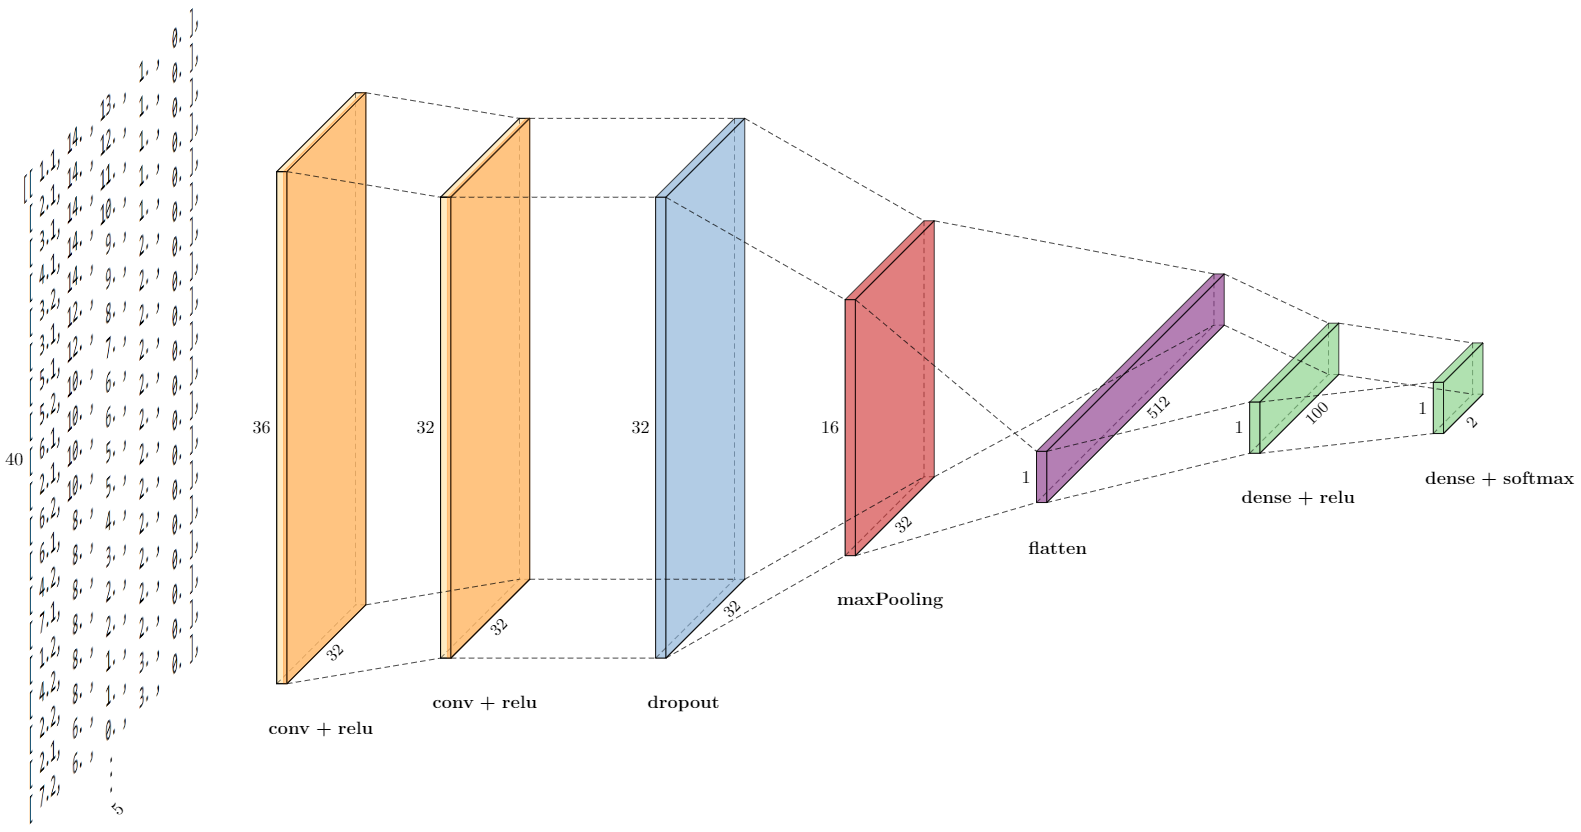
\includegraphics[width=15cm]{images/1dCnnStructure.png}
	\caption[Bild kurz]{Add caption}
	\label{fig:1dCnnStructure}
\end{figure}
\todo{anpassen an 1d cnn diagramm, weil es vorher falsch war}
The input data consist of the 5 statical features explained in .. \todo{ref} for each of the 40 steps (20 rounds), resulting in the input dimensions 40 $\cdot$ 4. Initially the data is passed to the first convolutional layer of the network. The first layer has 32 filters and the kernel has a size of 5, meaning that every step from the kernel includes all data from 5 steps in the game. This convolution results in 32 festure maps each with dimensions of 36 $\cdot$ 5. These feature maps are passed to the second convolutional layer with the same number of filters and the same kernel size as the first layer. This again results in 32 feature maps and a decresed dimensionality of 32 $\cdot$ 5. Afterwards a dropout layer with a rate of 0.5 randomly sets input units to 0 and by that helps to prevent overfitting. Then a one dimensional max pooling layer with a pool size of 2 reduces the dimensinalty to 16 $\cdot$ 5.  And finally the network is completed with a flatten layer and two dense layers \todo{vielleicht genauer erklären was dense macht, aber eigentlich ja oben auch schon, nur einen groben satz hier}. Both convolutional layers, and the first dense layer use a rectified linear unit as activation function. The last dense layer uses softmax normalization to bring the data down two two values for the two classes. The elemets of the output vector are between 0 and 1 and sum up to 1 and specify the result of the classification.  

\section{2D CNN}
The structure of the 1D CNN used is shown in figure \ref{fig:2dCnnStructure}.
\begin{figure}[H]
	\centering
	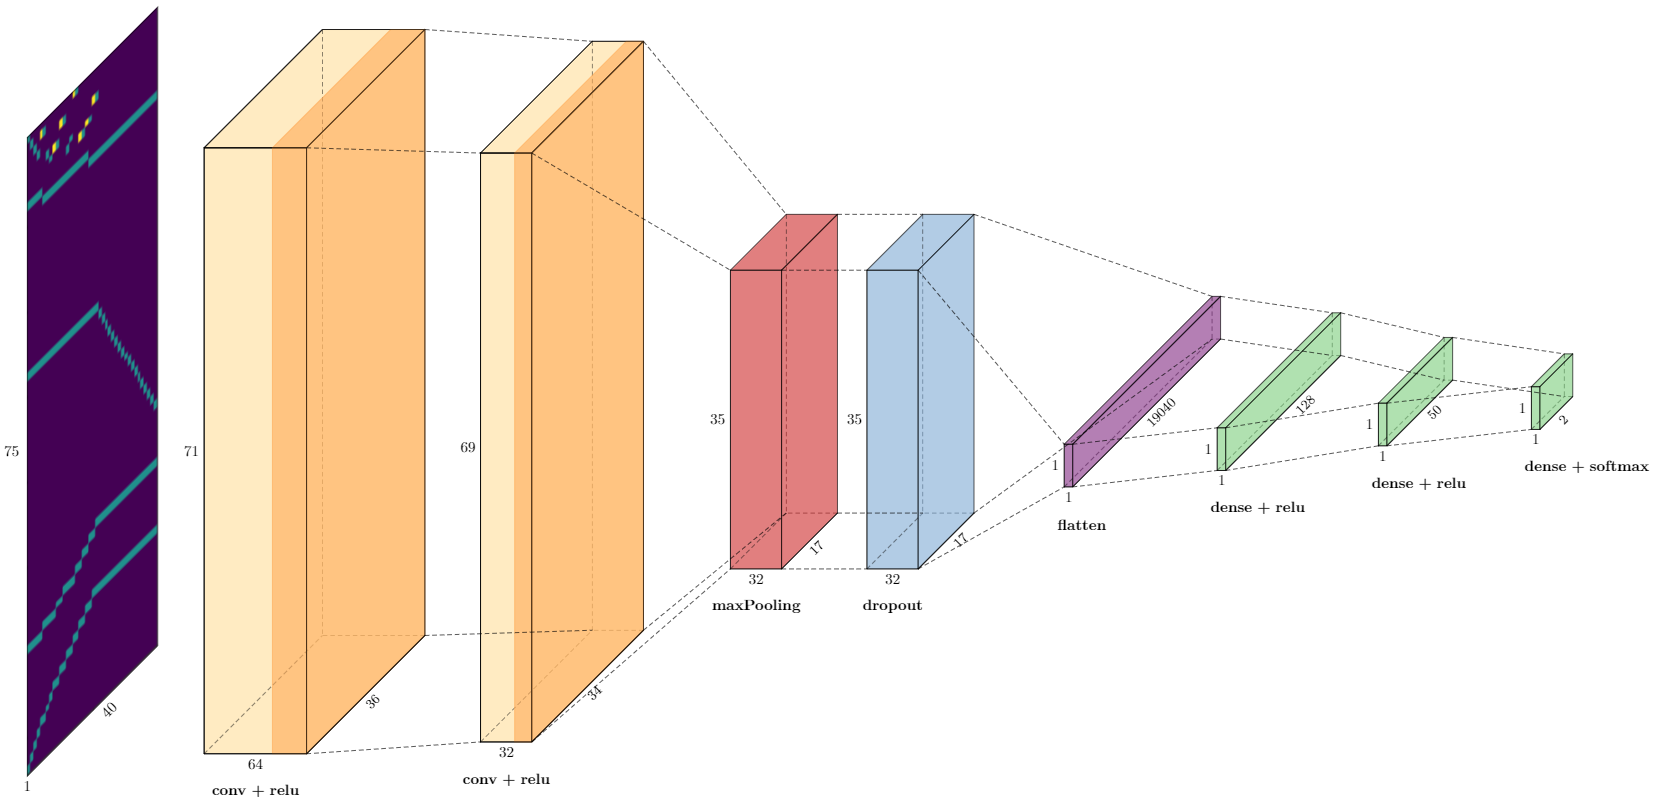
\includegraphics[width=15cm]{images/2dCnnStructure.png}
	\caption[Bild kurz]{Add caption}
	\label{fig:2dCnnStructure}
\end{figure}
The input data consist of the synthetic images generated in .. \todo{ref} using the 5 statistical features, resulting in the input dimensions 75 $\cdot$ 40. Initially the data is passed to the first convolutional layer of the network. The first layer has 64 filters and the kernel has a size of 5 $\cdot$ 5, meaning that each step from the kernel includes a 5 $\cdot$ 5 are of the synthetic image. This convolution results in 64 festure maps each with dimensions of 71 $\cdot$ 36. These feature maps are passed to the second convolutional layer with 32 filters and a kernel size of 3 $\cdot$ 3. This results in 32 feature maps and a decresed dimensionality of 69 $\cdot$ 34. Then a two dimensional max pooling layer with a pool size of 2 $\cdot$ 2 reduces the dimensinalty to 35 $\cdot$ 17. It is important to note that this does not happen by default. Due to the fact that 69 is odd, by default the last row would be ignored during a max pooling with dimensions 2 $\cdot$ 2 dimensions, meaning the dimensions would be 34 $\cdot$ 17 instead. As this is undesirable due to the potentially lost information in the last row, zero padding was used to create an additional row with zeros. This additional row results in the pooling not having to ignore the last row \todo{weil sich dimension auf 76 ändert stattdessen schreieb: da die height und width gerade sind und das pooling 2 mal 2 ist, wird beim pooling keine reihe oder spalte ausgelassen, es wird also kein zero padding benötigt}. Afterwards a dropout layer with a rate of 0.2 randomly sets input units to 0 and by that helps to prevent overfitting. And finally the network is completed with a flatten layer and three dense layers \todo{vielleicht genauer erklären was dense macht, aber eigentlich ja oben auch schon, nur einen groben satz hier}. Both convolutional layers, and the first two dense layers use a rectified linear unit as activation function. The last dense layer uses softmax normalization to bring the data down two two values for the two classes. The elements of the output vector are between 0 and 1 and sum up to 1 and specify the result of the classification.  


